% Highlighting elements in matrices
% Author: Stefan Kottwitz
\documentclass{article}
\usepackage{amsmath}
\usepackage{tikz}
\usetikzlibrary{fit,matrix}
\tikzset{%
  highlight/.style={rectangle,rounded corners,fill=red!15,draw,fill opacity=0.5,thick,inner sep=0pt}
}
\newcommand{\tikzmark}[2]{\tikz[overlay,remember picture,baseline=(#1.base)] \node (#1) {#2};}
%
\newcommand{\Highlight}[1][submatrix]{%
    \tikz[overlay,remember picture]{
    \node[highlight,fit=(left.north west) (right.south east)] (#1) {};}
}
\begin{document}
\[
\left(
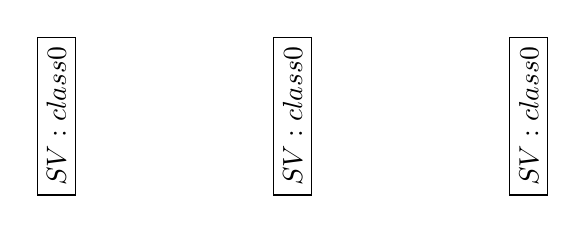
\begin{tikzpicture}[>=stealth,->,shorten >=2pt,looseness=.5,auto]
% in matrix of node mode, the content between the two vertical line |..| will pass to the cell node. 
\matrix [matrix of math nodes,
column sep={3cm,between origins},
%row sep={3cm,between origins},
nodes={rectangle, draw, minimum width=7ex}]
{
|[rotate=90](A)| SV:class 0  & |[rotate=90](A)| SV:class 0 & |[rotate=90](A)|  SV:class 0 \\
};
\end{tikzpicture}
\right)
\]
% \begin{tikzpicture}[>=stealth,->,shorten >=2pt,looseness=.5,auto]
% \matrix [matrix of math nodes,
% %column sep={2cm,between origins},
% %row sep={3cm,between origins},
% nodes={rectangle, draw, minimum width=7ex}]
% {
% & |(A)| A & \\
% |(B)| B & |(E)| E & |(C)| C \\
% & |(D)| D \\
% };
% \begin{scope}[every node/.style={font=\small\itshape}]
% \draw (A) to [bend left] node [midway] {g} (B);
% \draw (B) to [bend left] node [midway] {f} (A);
% \draw (D) -- node [midway] {c} (B);
% \draw (E) -- node [midway] {b} (B);
% \draw (E) -- node [near end] {a} (C);
% \draw (D) to [bend right, looseness=1]
% node [near start] {b} node [near end] {e} (A);
% \end{scope}
% \end{tikzpicture}
% \[
%   M = \left(\begin{array}{*3{c}}
%     \tikzmark{left}{$\cdot$} & \cdot  &  \\
%      &  &   \\
%      &  & \tikzmark{right}{}
%   \end{array}\right)
%   \Highlight[first]
%   \qquad
%   M^T = \left(\begin{array}{*5{c}}
%     \tikzmark{left}{1} & 6 & 11 & 16 \\
%     2 & 7 & 12 & 17 \\
%     3 & 8 & \tikzmark{right}{13} & 18 \\
%     4 & 9 & 14 & 19 \\
%     5 & 10 & 15 & 20
%   \end{array}\right)
% \]
% \Highlight[second]

% \tikz[overlay,remember picture] {
%   \draw[->,thick,red,dashed] (first) -- (second) node [pos=0.66,above] {Transpose};
%   \node[above of=first] {$N$};
%   \node[above of=second] {$N^T$};
% }
\end{document}​
%%% Local Variables: 
%%% mode: latex
%%% TeX-master: t
%%% End: 
